\documentclass{article}
\usepackage{polski}
\usepackage{amsfonts}
\usepackage{mathtools}

\DeclarePairedDelimiter\ceil{\lceil}{\rceil}
\DeclarePairedDelimiter\floor{\lfloor}{\rfloor}

\DeclareMathOperator*{\argmax}{arg\,max}
\DeclareMathOperator*{\argmin}{arg\,min}

\title{
    Bounded Diameter Minimum Spanning Tree \\
    \large Teoria Obliczeń i Złożoność Obliczeniowa
}
\author{Adrian Mucha}



\begin{document}

\maketitle

\cite{DBLP:journals/informaticaSI/PatvardhanPS15}
\section{Wprowadzenie}
Mając ważony, nieskierowany graf $G$ i dodatnią liczbę $D$ w problemie \textit{Bounded-Diameter Minimum Spanning Tree (BDMST)} szukamy najniższego kosztem drzewa rozpinającego spośród wszystkich drzew rozpinających $G$, których ścieżki składają się z co najwyżej $D$ krawędzi. Formalnie \textit{BDST} jest drzewem $T \subset E$ na $G = (V, E)$, którego średnica jest nie większa niż $D$. \textit{BDMST} ma na celu znalezienia drzewa rozpinającego o minimalnym koszcie $w(T) = \sum_{e\in T} w(e)$. Zawężając do grafów Euklidesowych, czyli takich w których wierzchołki są punktami na przestrzeni Euklidesowej a wagi krawędzi reprezentują dystans między parami wierzchołków nazywamy \textit{Euclidean BDMST}.

Problem BDMST jest NP-trudny dla $4 \leq D < |V| - 1$, oraz trudny w aproksymacji co motywuje w poszukiwaniach efektywnej strategii opartej na heurystykach, które potrafią szybko znaleźć BDST o niskim koszcie.

Oczywistym zastosowaniem \textit{EBDMST} jest znalezienie najtańszej sieci kabli lub rur by połączyć zbiór miejsc zakładając, że koszt połączenia zależny jest od jego długości.

%Innym zastosowaniem jest rozwiązanie aproksymacyjne Euklidesowego problemu Komiwojażera (\textit{Euclidean traveling salesman problem}). Realistycznie można rozwiązać ten problem 2-aproksymacją poprzez policzenie \textit{EBDMST} i poruszanie się po brzegu obejmującym całe drzewo.

\subsection{Definicja}
W książce \cite[p.~206]{10.5555/574848} Garey and Johnson pokazali, że Bounded Diameter Spanning Tree (BDST) problem jest NP-trudny.

Mając ważony graf nieskierowany $G = (V, E)$ oraz dwa parametry $D$ i $C$, decyzja \textit{czy drzewo rozpinające o koszcie $C$ oraz średnicy ograniczonej z góry przez $D$ istnieje} jest NP-zupełny. Jako pierwsi opisali ten problem i dowiedli NP-zupełności autorzy pracy \cite{DBLP:conf/compgeom/HoL89}.

Formalnie, mając graf $G$, funkcję kosztu $W(e) \in \mathbb{Z}^+, \forall_{e\in E}$, oraz nieujemne liczby całkowite $C$ i $D$, \underline{stwierdzić czy istnieje} drzewo rozpinające $T$, takie że $\sum_{e\in T} W(e) \leq C$ oraz $\sum_{e\in p} W(e) \leq D$ gdzie $p$ jest zbiorem wszystkich ścieżek w $T$. Ten problem nazywać będziemy Bounded Diameter Bounded Cost Spanning Tree (BDBCST).

\subsection{Przykłady}

Najprostszym grafem o zadanej maksymalnej średnicy $D$ drzewa rozpinającego jest \textit{graf liniowy} zawierający nie więcej niż $D + 1$ ($|V| \leq D + 1$, $|E| \leq D$) wierzchołków o funkcji kosztu $W(u, v) = \floor{\frac{D}{C}}$.

Przykładem negatywnym będzie więc graf w którym istnieje ścieżka między dwoma liśćmi dłuższa niż $D$, lub graf którego drzewo rozpinające zawiera krawędź $e_0$ której koszt przekracza ograniczenie $W(e_0) > C$.

\section{NP-zupełność}
\begin{theorem}
    BDBCST jest NP-zupełny

    \begin{proof}
        BDBCST jest NP. Najcięższą ścieżką musi być ścieżka łącząca dwa liście, więc możemy zgadnąć $n-1$ krawędzi i sprawdzić czy drzewo spełnia ograniczenia w czasie wielomianowym.
        
        Weźmy klauzule $C = \{C_1, C_2, \ldots, C_q\}$ z problemu \texttt{3SAT} na zbiorze zmiennych $\{X_1, X_2, \ldots, X_n\}$. Skonstruujemy graf $G = (V, E)$ i funkcję $W$ w taki sposób, że $C$ jest spełnialne wtedy i tylko wtedy gdy istnieje drzewo rozpinające $T$ dla grafu $G$, takie że $\sum_{e\in T} W(e) \leq 3n + 3q + 5$ oraz $\sum_{e\in p} W(e) \leq 10$ gdzie $p$ jest zbiorem ścieżek w drzewie $T$.

        $G$ konstruujemy w następujący sposób. $G$ zawiera następujące typy wierzchołków:
        \begin{itemize}
            \item ustanawiający prawdę wierzchołek $t$
            \item wierzchołki zmiennych $\{x_1, \bar{x}_1, x_2, \bar{x}_2, \ldots, x_n, \bar{x}_n\}$
            \item wierzchołki klauzul $\{c_1, c_2, \ldots, c_q\}$
            \item specjalny wierzchołek $s$
        \end{itemize}
        $G$ zawiera następujące krawędzie:
        \begin{itemize}
            \item krawędzie przypisania (waga $2$) $\{(t, x) | \forall x\}$
            \item krawędzie regulujące (waga $1$) $\{(x_i, \bar{x}_i) | i \in [1,n]\}$
            \item krawędzie powstrzymujące (waga $3$) $\{(u_i, c_j) | u_i = \begin{cases}
                x_i,        & \text{jeśli } X_i \in C_j\\
                \bar{x}_i,  & \text{jeśli }  \bar{X}_i \in C_j
            \end{cases}\}$
            \item krawędź $(t, s$) - waga $5$
        \end{itemize}
        Ta konstrukcja jest możliwa w czasie wielomianowym.

        \begin{figure}[h!]
            \centering
            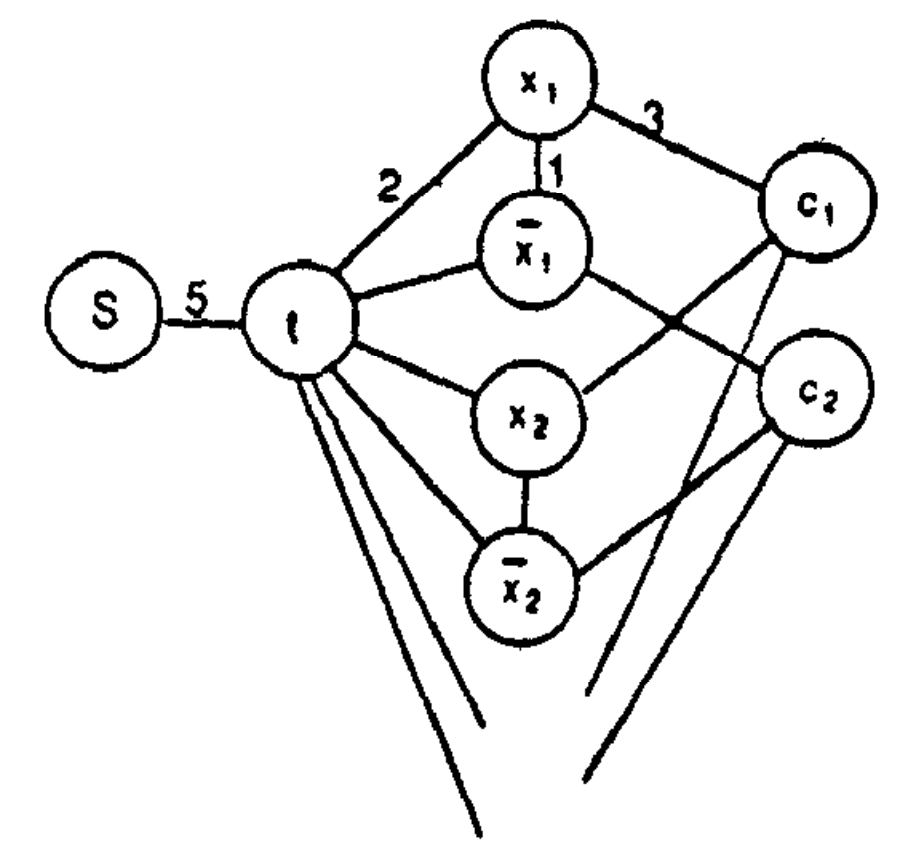
\includegraphics[width=0.5\textwidth]{graph_proof.png}
            \caption{Konstrukcja grafu $G$ w dowodzie twierdzenia 1}
            \label{fig:graph_proof_construct}
        \end{figure}

        Następnie załóżmy, że $C$ jest spełnialne. Istnieje więc przypisanie, takie że każda klauzula w $C$ zawiera conajmniej jeden prawdziwy literał. Możemy wybrać takie drzewo rozpinające $T$ składające się z następujących krawędzi:
        \begin{itemize}
            \item $(t, s)$
            \item $(t, x_i)$ dla każdego $i$ gdzie $X_i$ jest przypisany jako \texttt{TRUE} lub $(t, \bar{x}_i)$ w p.p.
            \item wszystkie krawędzie regulujące
            \item krawędzie powstrzymujące $(x_{i_j}, c_i)$, gdzie $X_{i_j}$ jest pierwszym literałem \texttt{TRUE} w klauzuli $C_i$.
        \end{itemize}
        Łatwo zauważyć, że $\sum_{e\in T} W(e) = 3n + 3q + 5$. Waga ścieżki od liścia do wierzchołka $t$ wynosi co najwyżej $5$, więc nie istnieje ścieżka w $T$ z wagą większą niż $10$.

        Załóżmy że mamy drzewo rozpinające $T$, takie że $\sum_{e\in T} W(e) \leq 3n +3q + 5$ oraz żadna ścieżka $p$ w $T$ nie jest dłuższa niż $10$. W $T$ jest $2n + q + 2$ wierzchołków i $2n + q + 1$ krawędzi. $T$ musi zawierać krawędź $(t, s)$, ponieważ $(t, s)$ jest jedyną krawędzią łączącą $s$. Wierzchołki klauzul są połączone jedynie za pomocą krawędzi powstrzymujących, a jest ich co najmniej $q$ w $T$. Załóżmy, że drzewo rozpinające $T$ składa się z $i$ krawędzi przypisania, $j$ krawędzi regulujących, $k + q$ krawędzi powstrzymujących oraz krawędzi $(t, s)$. Wtedy mamy
        \begin{align}
            i, j, k     &\geq 0 \\
            j           &\leq n \\
            i + j + k   &= 2n \\
            2i + j + 3k &\leq 3n 
        \end{align}
        Załóżmy, że $j < n$. Odejmując od (4) - $2\times (3)$, mamy $$k \leq j-n < 0$$, czyli sprzeczność. Ponadto, $T$ musi zawierać wszystkie $n$ krawędzi regulujących. Podstawiając $j = n$ otrzymujemy
        \begin{align}
            i + k   &= n \\
            2i + 3k &\leq 2n
        \end{align}
        Dalej odejmując od (6) - $2\times (5)$ otrzymujemy $k \leq 0$. Stąd $T$ zawiera dokładnie $q$ krawędzi powstrzymujących, $n$ krawędzi regulujących i $n$ krawędzi przypisania.

        Kolejno twierdzimy, że wszystkie wierzchołki klauzul sąsiadują tylko z tymi wierzchołkami zmiennych, które sąsiadują z wierzchołkiem $t$ w drzewie rozpinającym $T$. Teraz załóżmy, że to twierdzenie jest fałszywe. Ponieważ wierzchołki klauzul sąsiadują tylko z wierzchołkami zmiennych, musi więc istnieć wierzchołek ze zmienną $x$ oraz taki wierzchołek z klauzulą $c$, że $x$ sąsiaduje z $c$ ale nie sąsiaduje z $t$ w $T$ (patrz rysunek \ref{fig:graph_proof_construct}). Ścieżka z $c$ do $t$, która musi przebiegać przez $x$, ma więc wagę $6$. Ścieżka z $s$ do $c$ w $T$ musi wtedy ważyć $11$, co jest sprzeczne.

        Ponieważ $T$ zawiera wszystkie krawędzie regulujące, $T$ zawiera dokładnie jedną z krawędzi $(t, x_i)$ i $(t, \bar{x}_i)$ dla każdego $i$. Przypisując \texttt{TRUE} każdej zmiennej sąsiadującej z $t$ oraz \texttt{FALSE} ich zmiennym uzupełniającym, wszystkie klauzule w $C$ będą spełnione, ponieważ każda zawiera przynajmniej jeden prawdziwy literał. Stąd \texttt{3SAT} jest wielomianowo redukowalny do problemu $BDBCST$. 
    \end{proof}
\end{theorem}


\section{Podstawowe heurystyki}
Poniżej przedstawiono przegląd podstawowych heurystyk

\subsection{One-Time Tree Construction (OTTC)}

Jest to zachłanny algorytm oparty na heurystyce która oblicza średnicę drzewa rozpinającego w każdym kroku i upewnia się, że następny wierzchołek nie przekroczy ograniczenia. A następnie do budowanego drzewa rozpinającego w każdym kroku dodaje krwędź o najniższym koszcie, który nie łamie obostrzeń na średnicę. Dodanie wierzchołka wymaga pracy $\mathcal{O}(n^2)$, a całość wykonywana jest $n-1$ razy, więc całkowity czas pracy algorytmu rozpoczynającego w pojedynczym wierzchołku to $\mathcal{O}(n^3)$. Aby znaleźć najniższe kosztem BDST, algorytm OTTC uruchamiany jest dla każdego wierzchołka grafu ($n$ razy), więc całkowita złożoność wynosi $\mathcal{O}(n^4)$.

\subsection{Center-Based Tree Construction (CBTC)}
W drzewie o średnicy $D$, żaden wierzchołek nie nie znajduje się dalej niż $\frac{D}{2}$ skoków (lub krawędzi) od korzenia. Dzięki temu zabiegowi otrzymujemy szybszy algorytm bazujący na algorytmie Prima, który poprawia OTTC dzieki budowaniu BDST od środka drzewa. Zapamiętywanie stopnia wierzchołków i zapewnianie, że żaden nie przekroczy głębokości $\floor{\frac{D}{2}}$ pozwala zaoszczędzić ciągłego przeliczania średnicy drzewa przed dołączeniem wierzchołka do BDST. Otrzymujemy nieco lepszą złożoność $\mathcal{O}(n^3)$ w porównaniu do OTTC (tutaj również należy rozważyć algorytm startując z każdego wierzchołka osobno i wybrać drzewo o najniższym koszcie).

\subsection{Randomized Tree Construction (RTC)}
W losowej konstrukcji drzewa korzeń (centrum) jest wybierany na początku jako losowy wierzchołek (jeśli $D$ jest parzyste) lub losowane są dwa wierzchołki połączone ze sobą (jeśli $D$ jest nieparzyste). Każdy następny dołączany wierzchołek jest również wybierany losowo w sposób zachłanny, taki że przyłączenie wierzchołka nie przekroczy ograniczenia $D$ na średnicę drzewa. Jest to identyczny w implementacji algorytm jak CBTC z tą różnicą że wprowadzono element losowości przy wybieraniu wierzchołków. Również posiada tę samą złożoność $\mathcal{O}(n^3)$.

\subsection{Pozostałe heurystyki}
Po skonstruowaniu BDST jednym z algorytmów (CBTC lub RTC) dodatkowo sprawdzane jest dla każdego wierzchołka $v \in V$ którego głębokość jest większa niż $1$ czy można go odłączyć i połączyć z innym wierzchołkiem BDST mającym niższy stopień głębokości krawędzią o mniejszym koszcie.

Heurystyka przetrzymuje posortowaną macierz kosztów w celu szukania krawędzi o niskim koszcie by dodać do BDST wierzchołek $v$. Aby zachować kolejność, używa się macierzy pomocniczej pamiętającej indeksy \cite{DBLP:journals/soco/SinghG07}.

\section{Heurystyki CBLSoC-lite oraz CBLSoC}


\bibliographystyle{unsrt}
\bibliography{bdmst}

\end{document}
